\documentclass[a4paper]{article}

\usepackage[utf8x]{inputenc}
\usepackage[english]{babel}
\usepackage[a4paper,top=3cm,bottom=2cm,left=3cm,right=3cm,marginparwidth=1.75cm]{geometry}
\usepackage{amsmath}
\usepackage{bm} %bold for math formulas
\usepackage{amsfonts} %mathematical fields fonts
\usepackage{float} %images held
\usepackage[colorinlistoftodos]{todonotes}
\usepackage[colorlinks=true, allcolors=blue]{hyperref}
\usepackage[table]{colortbl}
\usepackage{multirow}
\usepackage{siunitx}
\usepackage{graphics}

\title{Integrazione di Sistemi Embedded\\Lab 07 Report}
\author{Matteo Perotti (251453)\\Giuseppe Puletto (251437)\\Luca Romani (255244)\\Giuseppe Sarda (255648)}


\begin{document}

\maketitle

\newpage

\begin{abstract}
	E' stato creato un sistema che si compone di due parti: un programma Python che viene eseguito da PC e un programma C caricato e fatto girare su scheda NUCLEO-F401RE. La comunicazione tra i due dispositivi avviene mediante un cavo USB che emula una seriale. 
	Il debug è stato eseguito grazie alla modalità di SEMIHOSTING che ha permesso il reindirizzamento dello std-output dal processore ARM Cortex M4 passando per il debugger/loader ST-LINK fino al PC.\newline
	La seguente relazione spiega i passi operativi in ordine temporale che hanno portato al progetto così come consegnato. La versione finale verrà descritta solo al capitolo 4
\end{abstract}

\section{Descrizione dell'algoritmo}
Le specifiche sono disponibili nel documento "lab07.pdf". Di seguito verranno chiarite le specifiche non definite:
\begin{enumerate}
	\item Qualora venga inviato un comando di accensione LED mentre esso è già acceso, il comando viene considerato non valido e semplicemente ignorato. Stessa cosa se il comando chiede di spegnere un LED già spento.
	\item E' necessario che dal PC i comandi arrivino nel formato corretto. Non devono essere inviati comandi più lunghi di due caratteri.
	\item Per ottenere un risultato corretto è indispensabile non attendere per più di 65 secondi dopo l'accensione/spegnimento del LED prima di premere il pulsante.
\end{enumerate}

\section{Programma Python}
Il programma Python, interfacciandosi tramite linea seriale col microcontrollore, permette di inviare o ricevere informazioni da quest'ultimo, informazioni quali i comandi per spegnere e accendere il led del micro o il tempo impiegato dall'utente per finire una simulazione. Pu\`{o} essere utilizzato sia tramite terminale che tramite interfaccia grafica. Il progetto Python+
3 consta di quattro file \textit{.py}: \textit{measurer.py}, \textit{lib.py}, \textit{constants.py} e \textit{gui.py}.

\subsection{Avvio - \textit{measurer.py}}
Il programma Python si avvia eseguendo il file \textit{measurer.py} e passandogli un parametro, ``-t" o ``-g". ``-t" permette l'esecuzione via terminale, mentre ``-g" quella via interfaccia grafica. Il file si serve oltre che delle librerie \textit{os} e \textit{sys}, del file \textit{lib.py}.
\newline 
Se \textit{measurer.py} viene eseguito passandogli un numero non corretto di parametri o un parametro diverso da ``-t" o ``-g", il programma segnala l'errore via terminale e termina con un exit status uguale a 2. Se avviato correttamente con l'opzione ``-g", \textit{measurer.py} esegue il file \textit{gui.py} e l'interfaccia grafica si apre.
\newline
Se avviato correttamente con l'opzione ``-t", \textit{measurer.py} interagisce con l'utente via terminale tramite un men\`{u}. L'utente pu\`{o} chiudere il programma o inviare il comando ``L0" (spegni il LED) o ``L1" (accendi il LED) digitando sul terminale rispettivamente q, y o n. Se si digita q, \textit{measurer.py} si chiude ritornando come exit state 0; se si digita y (n), \textit{measurer.py} esegue la funzione \textit{turn\_on\_LED\_terminal()} (\textit{turn\_off\_LED\_terminal()}) importata dal file \textit{lib.py}.  Il valore di ritorno di \textit{turn\_on\_LED\_terminal()} (\textit{turn\_off\_LED\_terminal()}) viene utilizzato come exit state al momento della chiusura del programma. Se si digita uno o pi\`{u} caratteri diversi dai tre prima specificati, il programma segnala l'errore via terminale, chiedendo nuovamente all'utente cosa voglia fare.

\subsection{Funzioni via terminale - \textit{lib.py}}
Il file \textit{lib.py} contiene la definizione delle funzioni \textit{delay\_cmd()}, \textit{send\_ser\_cmd(command\_to\_send)},  \textit{turn\_on\_LED\_terminal()} e \textit{turn\_off\_LED\_terminal()}, \\ \textit{t\_score\_byte\_object\_conversion\_to\_seconds} (\textit{t\_score\_byte\_object}).
\newline
La funzione \textit{turn\_on\_LED\_terminal()} (\textit{turn\_off\_LED\_terminal()}) invia alla porta seriale specificata nel file \textit{constants.py} il comando per accendere (spegnere) il led. Non riceve alcun parametro e ritorna un intero. Esso vale 3 se il LED \`{e} gi\`{a} acceso (spento), altrimenti ritorna 0.
\newline
La funzione \textit{send\_ser\_cmd(command\_to\_send)} riceve una stringa come parametro d'ingresso che contiene il comando che l'utente desidera inviare alla seriale; ritorna una stringa con il tempo impiegato dall'utente nel premere il pulsante o un errore; utilizza il pacchetto PySerial per gestire la comunicazione via seriale e le altre funzioni di \textit{lib.py} \textit{delay\_cmd()} e \textit{t\_score\_byte\_object\_conversion\_to\_seconds} (t\_score\_byte\_object).
\newline
Prima di tutto, \textit{send\_ser\_cmd()} apre la porta seriale e imposta baudrate, parity bit e byte size della comunicazione, nonch\'{e} un timeout per leggere la seriale. Il timeout \`{e} impostato a 100 s ed impedisce al programma Python di bloccarsi qualora dalla seriale non ricevesse i 5 byte che si aspetta. Poi, se il comando \`{e} valido, cio\'{e} il led è spento (acceso) e l'utente desidera accenderlo (spegnerlo), dopo un ritardo casuale di 10-20 secondi, viene inviato il comando sulla seriale, non prima per\'{o} di averlo convertito da stringa a una variabile di tipo byte. Dopo aver letto 5 byte dalla seriale, converte quanto ricevuto in stringa e la passa come parametro di ritorno. La funzione si preoccupa anche di aggiornare LED\_STATE, la variabile globale che permette al programma Python di ricordare lo stato del LED del micro. Qualora il comando non sia valido, ritorna come stringa un errore ``E0001" (``E0000") qualora si voglia accendere (spegnere) il led del micro che \`{e} gi\`{a} acceso (spento).
La funzione \textit{delay\_cmd()} n\'{e} riceve, n\'{e} ritorna alcun parametro. Usa la funzione \textit{randint} della libreria Python \textit{random} e \textit{sleep} della libreria Python time. Se eseguita, genera un ritardo casuale tra 10 e 20 secondi.
La funzione  \textit{t\_score\_byte\_object\_conversion\_to seconds} (\textit{t\_score\_byte\_object}) riceve una variabile byte come parametro d'ingresso e ritorna una stringa come parametro di ritorno. La variabile byte dovrebbe contenere il valore di un intervallo di tempo nella forma \textit{``Thhhh"}, dove \textit{``hhhh"} è il valore dell'intervallo di tempo in \textit{ms} espesso in esadecimale. Ritorna una stringa contenente il tempo convertito in millisecondi e la relativa unità di tempo. 

\subsection{File delle constanti - \textit{constants.py}}
Il file \textit{constants.py} contiene il valore delle costanti usate dai file \textit{.py}.
\subsection{Graphical user interface GUI}
L'interfaccia grafica è stata creata usando uno script in python e adoperando il modulo ``tkinter". La GUI consente all'utente di mandare i comandi ``L0" e ``L1" mediante l'utilizzo di due tasti presenti a schermo. Per quel che concerne l'utilizzo di funzioni e l'inizializzazione della porta seriale, l'interfaccia grafica si appoggia allo script lib.py.
\subsubsection{Widgets}
L'interfaccia grafica ha una finestra principale chiamata ``root" che viene creata mediante l'inizializzazione dell'interprete ``Tk()" del modulo di tkinter e al suo interno contiene gli oggetti:
\begin{itemize}
	\item main\_Frame
	\item led\_on
	\item led\_off
	\item quit\_button
	\item text\_score\_lab
	\item t\_score\_lab
	\item error\_lab
\end{itemize}
mainFrame è un frame che funziona da contenitore per i widget dell'interfaccia grafica. \`E stato istanziato per gestire in maniera separata il comportamento della finestra principale e dei widget.
Gli altri oggetti sopra elencati sono i widget dell'interfaccia grafica e in particolare:
\paragraph{led\_on} è un bottone verde che se premuto richiama la funzione turn\_on\_LED per inviare il comando ``L1" tramite la seriale alla scheda Nucleo. All'interno di questa funzione viene richiamata la funzione send\_ser\_command() di lib.py il cui valore di ritorno è salvato all'interno della variabile locale tmp. In base al valore di tmp la funzione turn\_on\_LED aggiorna t\_score con il nuovo tempo dell'utente oppure aggiorna il valore di error\_flag dell'etichetta error\_lab senza modificare t\_score.
\paragraph{led\_off} è un bottone grigio che consente all'utente, come il widget led\_on, di trasmettere il comando ``L0" tramite seriale per spegnere il LED della Nucleo richiamando la funzione turn\_off\_LED che lavora in modo speculare rispetto a quella dell'altro bottone.
\paragraph{quit\_button} è un bottone rosso che consente all'utente di uscire dal programma. Se premuto invoca la funzione ``quit()" dell'oggetto root che fa uscire lo script dal mainloop() dell'interfaccia grafica.
\paragraph{text\_score\_lab} è un'etichetta che contiene del testo (Your time score is).
\paragraph{t\_score\_lab} è un'etichetta che mostra il valore della variabile t\_score aggiornato in tempo reale.
\paragraph{error\_lab} è un'etichetta sensibile alla variabile error\_flag. 
\subsubsection{Struttura}
Per quello che riguarda il geometry manager si è deciso di adoperare ``pack()" per gestire mainFrame e ``grid()" per i vari widget. Dato che root ha un solo frame è stato usato pack(), in questo modo è stato più facile da configurare l'opzione di riempimento totale di mainFrame nella root e il suo ridimensionamento sempre in funzione della finestra padre. Al fine di ottenere questo risultato è stato necessario impostare in pack() i flag di ``expand" e ``fill" rispettivamente a ``BOTH" e ``1". Inoltre bisogna anche specificare quali righe e colonne del frame dovranno ridimensionarsi, per questo motivo sono stati inseriti due cicli for annidati che per ogni riga e ogni colonna vanno a mettere la variabile ``weight" delle funzioni ``rowconfigure()" e ``columnconfigure()" a 1. \newline
Avendo in totale cinque widget, si è scelto grid() per avere un'organizzazione di tipo matriciale della GUI, in seguito viene riportata la matrice dell'interfaccia:
\begin{table}[H]
	
	\renewcommand{\arraystretch}{3}
	
	\centering
	\begin{tabular}{l|c|c|c}
	     & 1 & 2 & 3 \\ \hline
		1  \qquad \qquad  &led\_on & \qquad & led\_off  \qquad \qquad \\ \hline
		2 & text\_score\_lab & t\_score\_lab & error\_lab \\ \hline
		3 & \qquad & quit\_button & \qquad
	\end{tabular}
\end{table}
\noindent
Anche per il manager grid è necessario cambiare delle variabili per ottenere un ridimensionamento automatico di ogni widget in funzione della finestra padre, di conseguenza è stata richiamata la funzione ``grid\_rowconfigure()" e ``grid\_columnconfigure" per andare a specificare quale riga e colonna dovessero essere ridimensionate dinamicamente. Per capire il fattore di scalamento del widget bisogna assegnare un valore alla variabile  ``weight" delle due funzioni sopra citate, in questo caso per tutti i widget, tranne il quit button, è stato scelto il valore 1.

\section{Programma C}
Il programma C deve permettere al microcontrollore di ricevere dati da seriale, interpretarli, accendere e spegnere un led, contare intervalli di tempo, formattarli e poi inviarli nuovamente tramite seriale.
	\subsection{CubeMX}
		Grazie al software CubeMX è stato possibile ottenere fin dall'inizio una struttura consistente del programma in modo molto agevole. 
		\paragraph{UART1} Dagli schematici è possibile vedere che il Cortex-M4 e l'ST-LINK sono collegati tramite seriale UART2. Per il programma è stata tuttavia usata UART1 per non passare dall'ST-LINK. Quest'ultima è collegata ai pins PA9 e PA10 del controllore principale e ai connettori D8 e D10 della scheda.
		In CubeMX è stato quindi selezionata l'USART1 e le impostazioni sono state regolate da specifiche; in aggiunta è stata selezionata anche l'inizializzazione degli interrupts relativi. Questo serve per poter gestire in modo non-blocking la ricezione e la trasmissione.
		\subparagraph*{Connessione fisica} La connessione per la trasmissione e ricezione dei comandi è stata effettuata tramite convertitore TTL-232R-3v3. Sono stati utilizzati tre connettori per assicurare un riferimento comune (cavo nero a GND), connettere RX della scheda (D2 - P10) a TX dell'adattatore (cavo arancione) e TX della scheda (D8 - P9) ad RX dell'adattatore (cavo giallo).
		\paragraph{TIM1} E' necessario contare con una risoluzione del millisecondo, ed il valore massimo esprimibile in tale unità di misura è 0xFFFF, ovvero 65,535 secondi. 
		Dal reference manual del microcontrollore è possibile vedere che il timer TIM1 è collegato ad APB2. Da CubeMX si può impostare il clock relativo affinché sia di 42 MHz, e il timer affinché il prescaler lo faccia scendere ancora fino ad 1 kHz. In questo modo viene evitata la creazione di una funzione di conversione apposita per ottenere il tempo in millisecondi a partire dal contenuto del registro del timer: con queste impostazioni essi si equivalgono.
		\paragraph{GPIO} Vengono usati il LED2 a disposizione dell'utente e il blue PushButton. Di quest'ultimo è importante attivare l'interrupt corrispondente allo stato di output asserito, ovvero al falling edge (si può ricavare dallo schematico che il pulsante cortocircuita a gnd il pin del microcontrollore).
		\paragraph{Clock settings}
		Come già spiegato nel precedente paragrafo è stato modificato il clock che arriva ad APB2. Il prescaler relativo è stato messo a 4. Il main clock è 84 MHz, viene quindi diviso per 4 per poi essere moltiplicato per 2 ed arrivare ad APB2.
	\subsection{Scrittura del programma}
		Il programma utilizza funzioni messe a disposizione dall'HAL della ST. Gli interrupt di ricezione e trasmissione UART, insieme con quello del push-button, sono stati astratti con tre funzioni callback.
		Per prima cosa sono definiti il buffer di trasmissione e ricezione (5 e 2 bytes rispettivamente).
		
		Prima del ciclo infinito viene chiamata la funzione \textbf{$HAL\_UART\_Receive\_IT$}, che abilita la ricezione in modalità non blocking con interrupt (è disponibile anche in modalità blocking, oppure con DMA).
		Tutto il resto del programma è implementato nelle funzioni di callback: non appena il buffer di ricezione è pieno viene eseguita quella di ricezione, che si occupa di fare il parsing del comando ricevuto a condizione che non sia già in corso una misurazione. Esso viene ignorato se non valido, mentre nel caso contrario viene eseguita l'azione corrispondente sul LED e viene avviato il timer. Un flag viene asserito per indicare che è in corso una misurazione, e un altra variabile indica se il LED è correntemente acceso o spento. In seguito viene ri-abilitata la ricezione dei dati da seriale.

		Quando il pulsante è premuto viene immediatamente salvato il valore attuale del counter in una variabile globale ed il timer viene fermato e resettato. Poi viene eseguito un controllo sul flag di misurazione: se non è asserito, allora l'azione viene ignorata. Altrimenti il flag di misurazione viene deasserito e il valore della variabile di supporto è convertito in esadecimale e formattato tramite la funzione sprintf su un'altra variabile temporanea. Con una funzione che implementa banalmente un ciclo for, questa "stringa" è copiata sul buffer di trasmissione senza il null character finale, per essere poi inviata tramite la funzione non-blocking \textbf{$HAL\_UART\_Transmit\_IT$}.
		Il controllo sul flag è eseguito successivamente al salvataggio del valore del counter per non introdurre un errore nel conteggio dovuto alla latenza delle operazioni di controllo.

		La funzione callback di fine trasmissione può non fare nulla ed è implementata con una \textbf{$\_\_NOP()$}.

	\subsection{Test e debug}
		Ogni periferico è stato testato singolarmente prima che venisse assemblato il programma. Il debug è stato eseguito mediante l'utilizzo della printf grazie alla modalità di semihosting; essa è stata implementata in una macro che riceve in ingresso una stringa che viene passata ad una printf ma con l'aggiunta di un carattere '\textbackslash n' finale. Come riportato sul sito della ST questa è una condizione necessaria per il corretto funzionamento del semihosting stesso.
		Per testare la seriale è stato utilizzato il programma minicom per inviare e ricevere caratteri.

		E' importante sottolineare come sia possibile accedere alla seriale ttyUSB0 solo se il file corrispondente non risulta bloccato per mancanza di permessi. Prima dell'esecuzione è necessario quindi assicurarsi che non ci siano restrizioni particolari sul file.
\section{Extra: la Leaderboard}
		Una volta aver soddisfatto le specifiche e testato in modo soddisfacente il sistema si è deciso di aggiungere una \textit{feature} extra alla parte "front end" del progetto e permettere all'utente di salvare il proprio \textit{score} in una leaderboard, la cui lunghezza può essere scelta all'interno del file \textit{constants.py}. \newline
		Al fine di implementare una classifica, accessibile e gestita mediante il programma, alcune modifiche sono state effettuate al codice e all'interfaccia grafica per:
		\begin{itemize}
			\item Dare l'opportunità di \textbf{aggiungere} il proprio punteggio alla \textit{leaderboard}.
			\item \textbf{Visualizzare} la classifica.
		\end{itemize}
		Nel caso l'utente voglia aggiungere lo \textit{score} ottenuto, deve identificarlo con un \textit{nickname}, richiesto dal programma, che verrà memorizzato e ordinato in modo crescente in base al punteggio. Se il nome scelto è gia presente in classifica, lo score verrà aggiornato solo se minore rispetto al precedente. Se non viene inserito il nome nessuna modifica viene effettuata.\newline
		Non è possibile azzerare la classifica mediante programma. Unico modo è quello di eliminare a mano il file di salvataggio contenuto nel path relativo \textit{./mem/MemCard1.txt} .
	\subsection{Esecuzione da terminale}
		L'esecuzione da terminale si presenta come segue:

		\begin{figure}[H]
			\centering
			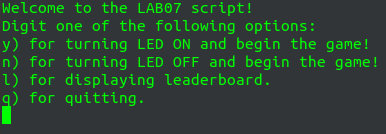
\includegraphics[scale=0.75]{img/terminal.png}
			\caption{Menù programma da terminale}
		\end{figure}
		Digitando l'opzione \textbf{\textit{l}} è possibile stampare a schermo la classifica.
		Nel caso invece si avvii il gioco e si ottenga un punteggio valido, il programma chiede se si vuole salvare. In caso affermativo viene richiesto il \textit{nickname} da associare allo score.
	\subsection{Esecuzione con GUI}
		L'esecuzione con GUI si presenta come segue:
		\begin{figure}[H]
			\centering
			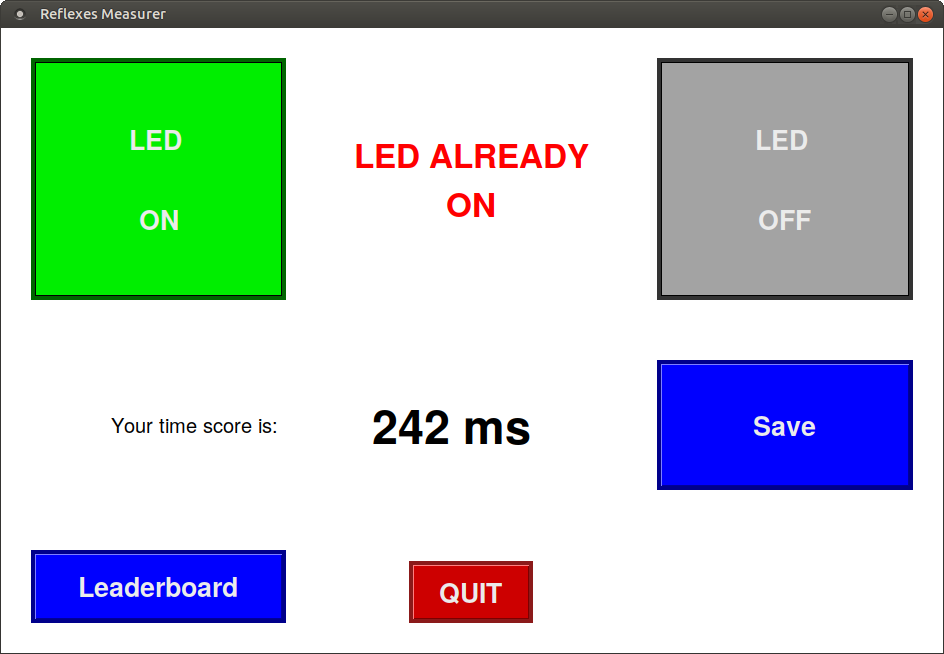
\includegraphics[scale=0.35]{img/GUI.png}
			\caption{Interfaccia grafica del programma}
		\end{figure}
		Dove, rispetto alla precedente versione, l'errore è stato posizionato tra i due pulsanti di avvio.
		Al suo posto è stato inserito il \textit{Button} che permette all'utente di salvare il punteggio. Una volta premuto farà aprire la seguente finestra:
		\begin{figure}[H]
			\centering
			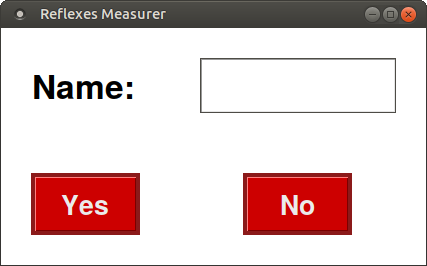
\includegraphics[scale=0.35]{img/save.png}
			\caption{Finestra di salvataggio}
		\end{figure}
		Dove se si preme il pulsante "\textbf{Yes}" il \textit{Name:} inserito viene salvato insieme al punteggio nel file di memoria, e poi la finestra viene chiusa. Diversamente, premendo "\textbf{No}" nessuna operazione viene effettuata se non il ritorno alla interfaccia principale.\newline
		Secondo \textit{Button} inserito è quello relativo alla visualizzazione della classifica vera e propria. Se viene premuto la finestra di dialogo che si aprirà è la seguente:
		\begin{figure}[H]
			\centering
			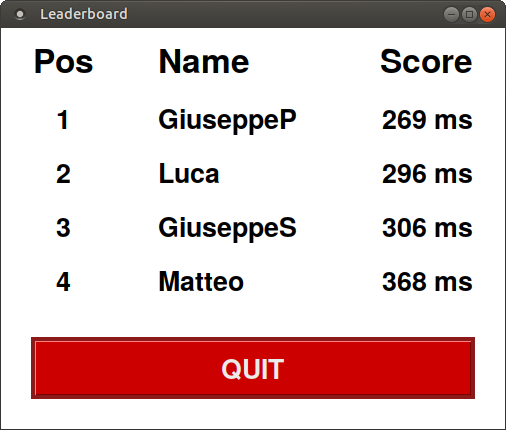
\includegraphics[scale=0.35]{img/leaderboard.png}
			\caption{Leaderboard}
		\end{figure}
	\section{Limiti del progetto}
		Principali limiti del progetto sono maggiormente due.\newline
		\begin{itemize}
			\item Il primo è relativo alla UART la quale, al primissimo avvio del gioco dopo il reset o il caricamento del programma, a volte invia un dato inesatto che non si aspetta. Dalla seconda esecuzione tutto funziona correttamente.
			\item Altro limite del programma è il fatto che al suo avvio si presuppone il LED sia spento. Ma se all'esecuzione precedente, si è chiusa l'interfaccia con il LED ancora acceso,  all'avvio successivo del programma bisognerà premere il bottone \textit{LED ON}, attendere i 100s di timeout e poi tutto riprende normalmente.
			Alternativa, in tale caso, è premere il tasto nero di reset sul micro controllore.
		\end{itemize}
		
\end{document}
